% Fig 1b - JEPA as a partitioned block diagram (physical | computational),
% in the style of a data-driven control schematic, for a fluids audience.
% Parallel: the encoder is the state representation; the predictor is the
% forward (world) model that replaces an RL actor/critic. No decoder in training.
% Standalone-compilable: pdflatex fig1b_jepa_blockdiagram.tex

\documentclass[border=10pt,tikz]{standalone}
\usepackage{tikz}
\usepackage{amsmath,amssymb}
\usetikzlibrary{positioning,arrows.meta,fit,backgrounds,calc}

\begin{document}
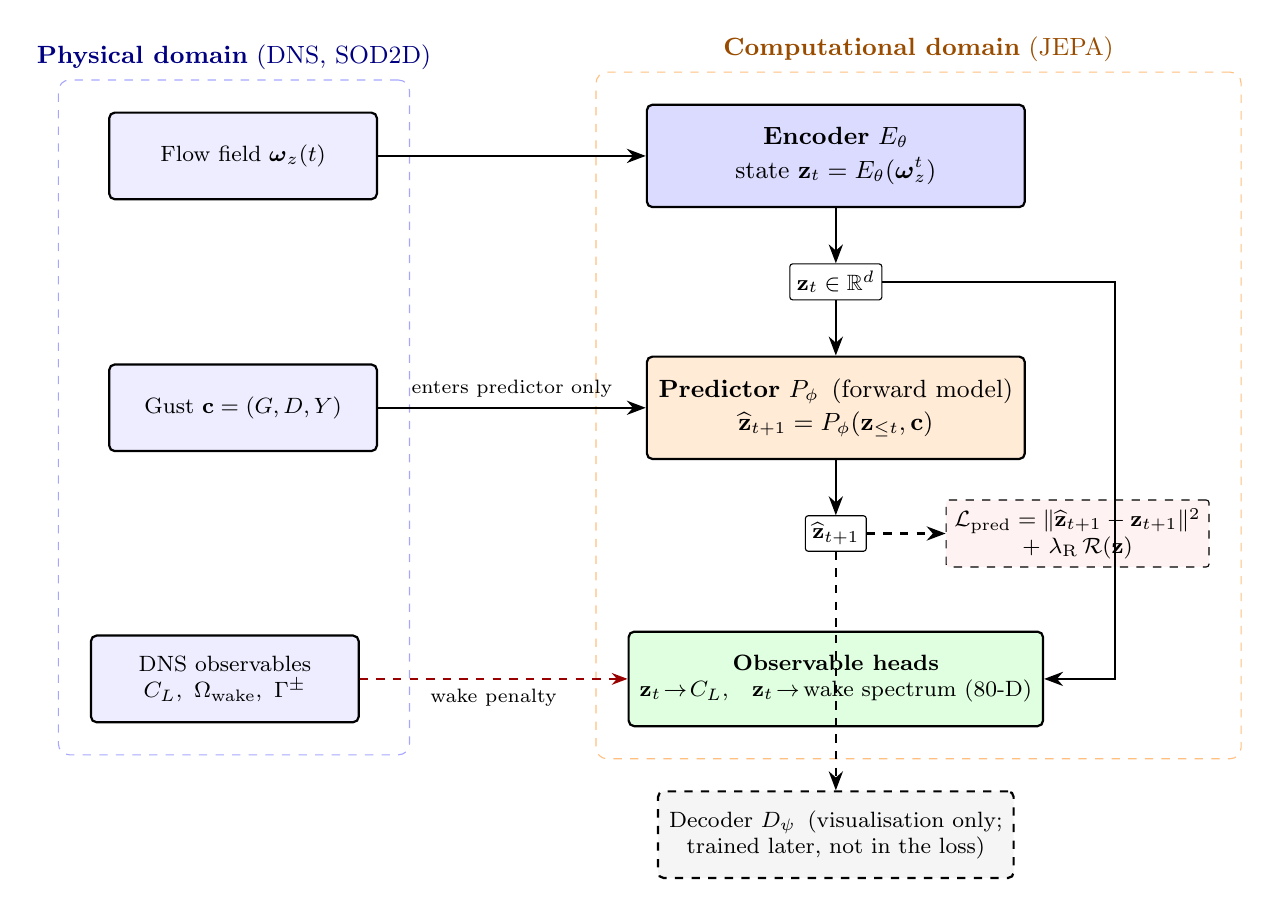
\begin{tikzpicture}[
    font=\small,
    box/.style={draw, rounded corners=2pt, align=center, inner sep=4pt, thick},
    phys/.style={box, fill=blue!7,  minimum width=34mm, minimum height=11mm, font=\footnotesize},
    enc/.style={box, fill=blue!14,  minimum width=48mm, minimum height=13mm},
    pred/.style={box, fill=orange!16, minimum width=48mm, minimum height=13mm},
    head/.style={box, fill=green!12, minimum width=48mm, minimum height=12mm, font=\footnotesize},
    st/.style={draw, rounded corners=1pt, fill=white, inner sep=2.5pt, font=\footnotesize},
    dec/.style={box, dashed, fill=gray!8, minimum width=44mm, minimum height=11mm, font=\footnotesize},
    los/.style={draw, dashed, rounded corners=1pt, fill=red!5, align=center,
                inner sep=3pt, font=\footnotesize},
    arr/.style={-{Stealth[length=2.4mm]}, thick},
    sup/.style={-{Stealth[length=2mm]}, dashed, semithick, red!60!black},
  ]

  % ===== computational spine (right) =====
  \node[enc] (E)
    {\textbf{Encoder} $E_{\theta}$\\[1pt] state $\mathbf{z}_t=E_{\theta}(\boldsymbol{\omega}_z^{t})$};
  \node[st, below=7mm of E] (zt) {$\mathbf{z}_t\in\mathbb{R}^{d}$};
  \node[pred, below=7mm of zt] (P)
    {\textbf{Predictor} $P_{\phi}$ \,(forward model)\\[1pt]
     $\widehat{\mathbf{z}}_{t+1}=P_{\phi}(\mathbf{z}_{\le t},\mathbf{c})$};
  \node[st, below=7mm of P] (zhat) {$\widehat{\mathbf{z}}_{t+1}$};
  \node[head, below=10mm of zhat] (H)
    {\textbf{Observable heads}\\ $\mathbf{z}_t\!\to\!C_L$,\quad $\mathbf{z}_t\!\to\!$ wake spectrum (80-D)};

  \node[los, right=10mm of zhat] (Lp)
    {$\mathcal{L}_{\mathrm{pred}}=\lVert\widehat{\mathbf{z}}_{t+1}-\mathbf{z}_{t+1}\rVert^2$\\
     $+\ \lambda_{\mathrm R}\,\mathcal{R}(\mathbf{z})$};
  \node[dec, below=8mm of H] (D)
    {Decoder $D_{\psi}$ \,(visualisation only;\\ trained later, not in the loss)};

  % ===== physical / DNS domain (left), aligned with their targets =====
  \node[phys, left=34mm of E] (omega) {Flow field $\boldsymbol{\omega}_z(t)$};
  \node[phys, left=34mm of P] (gust) {Gust $\mathbf{c}=(G,D,Y)$};
  \node[phys, left=34mm of H] (obsv) {DNS observables\\ $C_L,\ \Omega_{\mathrm{wake}},\ \Gamma^{\pm}$};

  % ===== arrows =====
  \draw[arr] (omega.east) -- (E.west);
  \draw[arr] (E) -- (zt);
  \draw[arr] (zt) -- (P);
  \draw[arr] (P) -- (zhat);
  \draw[arr] (gust.east) -- (P.west)
        node[midway, above, font=\scriptsize]{enters predictor only};
  \draw[arr] (zt.east) -| ($(H.east)+(9mm,0)$) |- (H.east);   % z_t feeds the heads
  \draw[arr, dashed] (zhat.east) -- (Lp.west);
  \draw[sup] (obsv.east) -- (H.west)
        node[midway, below, font=\scriptsize, black]{wake penalty};
  \draw[arr, dashed] (zhat) -- (D);

  % ===== domain frames =====
  \begin{scope}[on background layer]
    \node[draw=blue!35, dashed, rounded corners=4pt, inner sep=4mm,
          fit=(omega)(gust)(obsv),
          label={[blue!50!black]above:\textbf{Physical domain} (DNS, SOD2D)}] {};
    \node[draw=orange!50, dashed, rounded corners=4pt, inner sep=4mm,
          fit=(E)(zt)(P)(zhat)(H)(Lp),
          label={[orange!60!black]above:\textbf{Computational domain} (JEPA)}] {};
  \end{scope}

\end{tikzpicture}
\end{document}
